\documentclass[a4paper,11pt]{article}
\pdfoutput=1

\usepackage[T1]{fontenc}
\usepackage[utf8]{inputenc}
\usepackage{amsmath}
\usepackage{amssymb}
\usepackage{siunitx}
\usepackage{booktabs}
\usepackage{array}
\usepackage{graphicx}
\usepackage{jheppub}

\graphicspath{{figs/}}
\sisetup{detect-all, table-number-alignment=center, table-align-text-post=false}

\title{Agnostic search for a vector-like top partner at a lepton collider via the recoil mass technique}

\author[a]{Higinio Valle}
\author[a]{Cristina Oropeza Barrera}
\author[a]{Oscar Ochoa-Valeriano}

\affiliation[a]{Universidad Iberoamericana Ciudad de Mexico,
Prolongacion Paseo de la Reforma 880, Col. Lomas de Santa Fe, Alvaro Obregon,
Mexico City 01219, Mexico}

\emailAdd{cristina.oropeza@ibero.mx}

\abstract{A prospective study of single production of a vector-like top partner
$T$ at a $\sqrt{s}=\SI{3}{TeV}$ $e^+e^-$ collider is presented using a recoil-mass
strategy against a hadronically reconstructed Standard Model top candidate.  The
analysis is reframed as a two-level study: an idealized recoil proof of concept
based on unpolarized samples without ISR, and a CLIC-motivated stress test with
ISR and electron-beam polarization.  The simulated samples are generated with
\textsc{MadGraph5\_aMC@NLO}, decayed with \textsc{MadSpin}, showered with
\textsc{Pythia}~8, and processed through a custom \textsc{FastJet}-based
reconstruction.  No GEANT4/CLICdet full simulation or $\gamma\gamma\to$hadrons
overlay is assumed for the quoted reach.  The paper documents the object
definitions, background coverage, width validity domain, and statistical
treatment needed to make the recoil technique reproducible.  The resulting
$(m_T,\kappa_T)$ interpretation is therefore presented as a transparent
decay-agnostic baseline and as a roadmap for a full CLIC-realistic analysis.}

\keywords{Vector-like quarks, Electron-positron collider, Recoil mass, CLIC}

\begin{document}
\maketitle
\flushbottom
\tableofcontents
\clearpage

\section{Introduction}

Vector-like quarks (VLQs) are common in extensions of the Standard Model in
which the top sector participates in stabilizing the electroweak scale.  Their
decay patterns depend on the electroweak representation and on model-specific
mixing assumptions.  This model dependence is a persistent limitation of
channel-optimized LHC searches: a selection designed for one branching-fraction
hypothesis can lose efficiency when the same state decays through a different
mixture of $Wb$, $Zt$, and $Ht$ final states.

A multi-TeV $e^+e^-$ collider provides a complementary handle.  The known
initial state allows one to reconstruct the recoil mass against the associated
Standard Model top quark in $e^+e^-\to T\bar t$ or its charge conjugate.  The
central idea is not to reconstruct the full $T$ decay.  Instead, one selects a
boosted hadronic top candidate and asks whether the system recoiling against it
is compatible with a heavy object.  This can preserve sensitivity across decay
modes, provided the top candidate is selected robustly and machine effects are
treated honestly.

The revised analysis therefore separates what is already demonstrated from what
requires further simulation.  The present ROOT samples support an idealized
proof of concept and ISR/polarization stress tests.  They do not support the
claim of a final full-simulation CLIC reach.  The manuscript consequently
removes that claim, documents the assumptions entering the current result, and
defines the additional studies needed for a JHEP-level CLIC-realistic
projection.

\section{Signal and background samples}
\label{sec:samples}

The signal model follows the model-independent top-partner framework of
Ref.~\cite{Buchkremer:2013bha}.  The effective coupling $\kappa_T$ controls the
single-production rate, while the benchmark branching pattern used in the
inclusive samples is $T\to Wb$, $T\to Zt$, and $T\to Ht$ in the usual singlet
ratio.  The benchmark masses are
$m_T=\{1.2,1.6,2.0,2.4\}\,\si{TeV}$, with dedicated samples generated for the
available $\kappa_T$ points.

\begin{figure}[t]
\centering
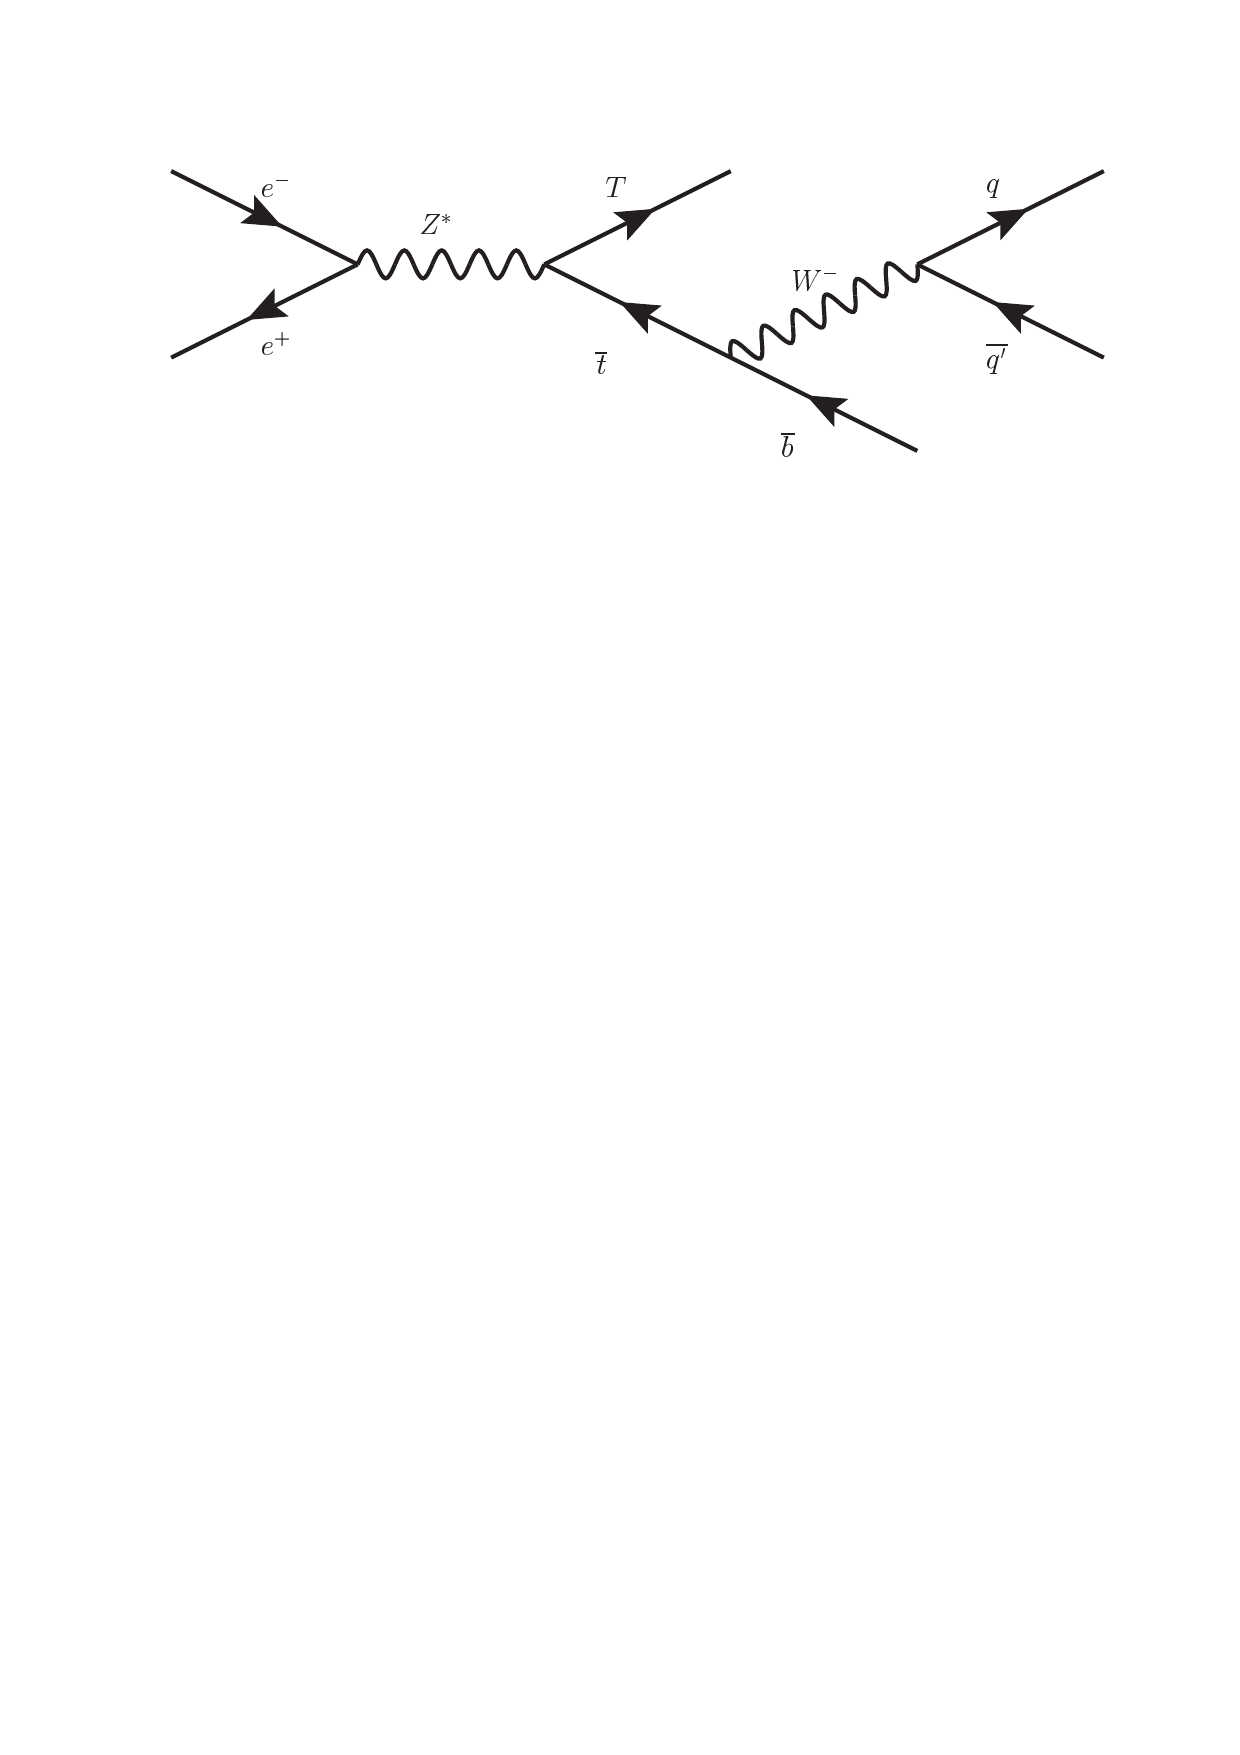
\includegraphics[width=0.55\textwidth]{feynman_diagram.png}
\caption{Representative single-production topology for the vector-like top
partner.  The analysis reconstructs the associated hadronic top and uses the
mass recoiling against that candidate.}
\label{fig:feynman}
\end{figure}

The current samples were generated at tree level with
\textsc{MadGraph5\_aMC@NLO}~\cite{Alwall:2014hca}, decayed with
\textsc{MadSpin}~\cite{Artoisenet:2012st}, and showered with
\textsc{Pythia}~8~\cite{Sjostrand:2014zea}.  They are then processed through the
custom analysis code in this repository.  Table~\ref{tab:reproducibility}
summarizes the reproducibility information that fixes the interpretation of the
quoted numbers.

\begin{table}[t]
\centering
\caption{Reproducibility record for the revised interpretation of the reviewed
samples.  The final CLIC-realistic reach must replace the missing entries before
being presented as a detector-level projection.}
\label{tab:reproducibility}
\begin{tabular}{p{0.28\linewidth} p{0.62\linewidth}}
\toprule
Item & Value used in the current revision \\
\midrule
Collider setup & $\sqrt{s}=\SI{3}{TeV}$, $L=\SI{5}{ab^{-1}}$; unpolarized, ISR-only, ISR+$P_{e^-}=\pm80\%$, and fresh CLIC luminosity-spectrum samples are kept separate. \\
Event generation & \textsc{MadGraph5\_aMC@NLO} local tree, \textsc{MadSpin} decays, \textsc{Pythia}~8 showering. \\
Beam treatment & The fresh CLIC production samples the luminosity spectrum through event-by-event beam-energy fractions and is compared to the older ISR-only lepton-beam setup. \\
Overlay treatment & A parametric one-bunch $\gamma\gamma\to$hadrons overlay stress test is reconstructed for the fresh CLIC samples. \\
Detector treatment & Custom \textsc{FastJet}-based object reconstruction; no GEANT4/CLICdet full simulation and no Delphes card are used for the quoted fast/parametric reach. \\
Main histogram & \texttt{mrecoil\_isolated\_toplikes\_rec\_missE\_cut}. \\
Normalization & ROOT metadata histograms \texttt{Cross\_Section} and \texttt{no\_sim}, scaled to $L=\SI{5}{ab^{-1}}$. \\
Nominal fiducial region & The revised analysis code defaults reconstructed objects to $|\eta|<2.5$; legacy figures from the reviewed PDF used $|\eta|<5$ and are explicitly treated as validation inputs pending rerun. \\
\bottomrule
\end{tabular}
\end{table}

\begin{table}[t]
\centering
\caption{Background treatment in the revision.  The fresh CLIC production now
includes the original four generated background classes with ISR, luminosity
spectrum, and a parametric one-bunch $\gamma\gamma\to$hadrons overlay stress
test.  Additional electroweak and high-mass inclusive backgrounds remain
required before claiming a final detector-level CLIC reach.}
\label{tab:background-status}
\small
\begin{tabular}{@{}p{0.34\linewidth}p{0.24\linewidth}p{0.32\linewidth}@{}}
\toprule
Class & Status & Revision use \\
\midrule
$t\bar t$, $t\bar t Z$, $t\bar t H$, $W^+W^-Z$ & Fresh CLIC rerun complete & Used in Tables~\ref{tab:fresh-clic-reach}--\ref{tab:fresh-clic-vs-isr} \\
$\gamma\gamma\to$ hadrons overlay & Parametric stress test complete & One-bunch overlay impact reported in Table~\ref{tab:fresh-clic-overlay} \\
$t\bar t\nu\bar\nu$, $W^+W^-\nu\bar\nu$, $H\nu\bar\nu$, $ZZ$, $HZ$, $W^+W^-$ & Present in local analysis tree or queued as auxiliary inputs & Add to expanded-background rerun before final reach claim \\
W-fusion single top and high-mass $V+$jets & Not yet generated & Require generation or data-driven upper bound \\
\bottomrule
\end{tabular}
\end{table}


The background table distinguishes samples included in the fresh CLIC rerun,
the overlay stress-test treatment, locally available auxiliary backgrounds, and
processes that must still be generated or bounded before claiming a full
detector-level CLIC sensitivity.  This distinction is essential because missing
W-fusion single-top and high-mass inclusive backgrounds can directly affect the
recoil-mass tails.

\section{Event selection and reconstruction}
\label{sec:selection}

The recoil mass is computed as
\begin{equation}
  m_{\rm recoil}^{2}
  = s - 2 E_{\rm top}\sqrt{s} + m_{\rm top}^{2},
  \label{eq:recoilmass}
\end{equation}
where $E_{\rm top}$ and $m_{\rm top}$ are reconstructed from the selected
large-radius top candidate.  The calculation uses the nominal collision energy,
which is why ISR and beamstrahlung are expected to broaden the distribution.

The object definitions are fixed as follows.  Stable visible particles are
clustered with the Cambridge--Aachen algorithm.  Small-radius jets use $R=0.5$
and $p_T>\SI{20}{GeV}$; large-radius jets use $R=1.0$ and
$p_T>\SI{100}{GeV}$.  The current code now defaults reconstructed objects to
$|\eta|<2.5$ for the nominal revision.  The legacy reviewed plots are kept only
as the pre-revision $|\eta|<5$ comparison until the full rerun is completed.

The large-radius jet is passed to the Johns Hopkins top tagger
\cite{Kaplan:2008ie} with
\[
  (\delta_p,\delta_r,\cos\theta_W^{\rm max})=(0.03,0.11,0.7),
\]
a top mass window of $\SIrange{150}{200}{GeV}$, and a $W$ mass window of
$\SIrange{65}{95}{GeV}$.  A truth-level $b$-matching requirement is applied by
requiring the non-$W$ subjet to lie within $\Delta R<0.4$ of a generated
$b$-quark.  This is not an experimental b-tag model; the final detector-level
study must replace it with efficiency and mistag parameterizations.

The isolation and misassignment veto are also defined explicitly.  Isolated
electrons and muons are identified with a mini-isolation cone
$R_{\rm iso}=10/p_T^\ell$ and a hadronic activity ratio threshold of 0.1.
For each top-tagged large-radius jet, the code counts nearby small jets with
$p_T>\SI{25}{GeV}$ and $1.7<\Delta R({\rm large}\mbox{-}R,{\rm small}\mbox{-}R)<2.5$,
and nearby isolated leptons with $p_T>\SI{25}{GeV}$ and $\Delta R<2.5$.
The nearby-activity veto is applied in the current implementation when the
selected large-radius jet carries a relative transverse momentum
$p_T^{\rm largeR}/H_T>0.4$, where $H_T$ is the scalar $p_T$ sum of the small-$R$
jets.  The final selection then requires
\[
  m_{\rm recoil}>\SI{1.1}{TeV},\qquad E_{\rm miss}<\SI{1}{TeV}.
\]

\section{Statistical treatment}
\label{sec:statistics}

The reviewed paper quoted $S/\sqrt{S+B}$ counting significances.  The revised
workflow keeps that number only as a diagnostic and uses a binned
profile-likelihood test over the recoil-mass spectrum as the headline
statistical model.  The local discovery utility now uses an explicit manual
binned profile-likelihood closure as the authoritative asymptotic result.  The
RooStats backend is kept only as a diagnostic because the local zero-nuisance
configuration can return the known invalid $p_0=0.5$ result.  The closure
condition is that an Asimov signal-plus-background dataset gives a nonzero
discovery significance and that the nuisance-free binned result agrees with the
manual Cowan-Asimov calculation~\cite{Cowan:2010js}.

The paper also reports transparent counting cross-checks with systematic
uncertainties.  The $5\%$ background-normalization scenario uses the standard
Gaussian-constrained Cowan expression.  The $10\%$ background plus $5\%$
signal-efficiency column is deliberately conservative: the signal yield is
shifted down by one efficiency uncertainty before evaluating the constrained
counting significance.  These columns are not substitutes for the final binned
nuisance model, but they expose how rapidly the current inclusive counting
reach degrades under realistic normalization uncertainties.

\begin{table}[t]
\centering
\caption{Binned profile-likelihood closure for the unpolarized fresh CLIC
samples.  The recoil histograms use the mass-matched BDT selections and are
rebinned to $\SI{100}{GeV}$ bins to avoid empty-background template bins.  The
agreement between $Z_{\rm binned}$ and $Z_{\rm PLR}^{\rm Asimov}$ validates the
manual profile-likelihood implementation for these inputs.}
\label{tab:fresh-clic-profile}
\small
\begin{tabular}{lrrrrrr}
\toprule
$m_T$ [TeV] & $S$ & $B$ & $Z_A^{\rm count}$ & $Z_A^{\rm binned}$ & $Z_{\rm PLR}^{\rm Asimov}$ & $Z(5\%B)$ \\
\midrule
    1.2 & 178.2 & 10278.4 & 1.75 & 1.91 & 1.91 & 0.34 \\
    1.6 & 129.5 & 6404.3 & 1.61 & 2.03 & 2.03 & 0.39 \\
    2.0 & 64.6 & 5052.5 & 0.91 & 1.17 & 1.17 & 0.25 \\
    2.4 & 13.5 & 4325.7 & 0.21 & 0.39 & 0.39 & 0.06 \\
\bottomrule
\end{tabular}
\end{table}


\section{Baseline and realism stress tests}
\label{sec:realism}

\subsection{Idealized recoil calibration}

The unpolarized, no-ISR samples are used only to calibrate the intrinsic
recoil-mass behavior.  Table~\ref{tab:cutflow} reproduces the reviewed cutflow
for $m_T=\SI{1.2}{TeV}$ and $\kappa_T=0.20$.  It is labeled as an idealized
legacy acceptance result because the corresponding ROOT files were produced
with the pre-revision $|\eta|<5$ acceptance.

\begin{table}[t]
\centering
\caption{Reviewed baseline cutflow for the $m_T=\SI{1.2}{TeV}$, $\kappa_T=0.20$
signal and the dominant $t\bar t$ background, scaled to $\SI{5}{ab^{-1}}$.
This table is retained as the idealized calibration sample; the nominal
detector-fiducial rerun uses $|\eta|<2.5$.}
\label{tab:cutflow}
\begin{tabular}{lrr}
\toprule
Selection step & Signal & $t\bar t$ \\
\midrule
All events & 1232.3 & 95706.0 \\
Fat-jet preselection & 1232.0 & 95335.1 \\
Top tagged & 401.4 & 41535.0 \\
Substructure tag & 348.6 & 37869.4 \\
Isolation veto & 215.1 & 31975.5 \\
$m_{\rm recoil}>\SI{1.1}{TeV}$ & 206.1 & 5897.1 \\
$E_{\rm miss}<\SI{1}{TeV}$ & 198.6 & 5654.6 \\
\bottomrule
\end{tabular}
\end{table}

\begin{figure}[t]
\centering
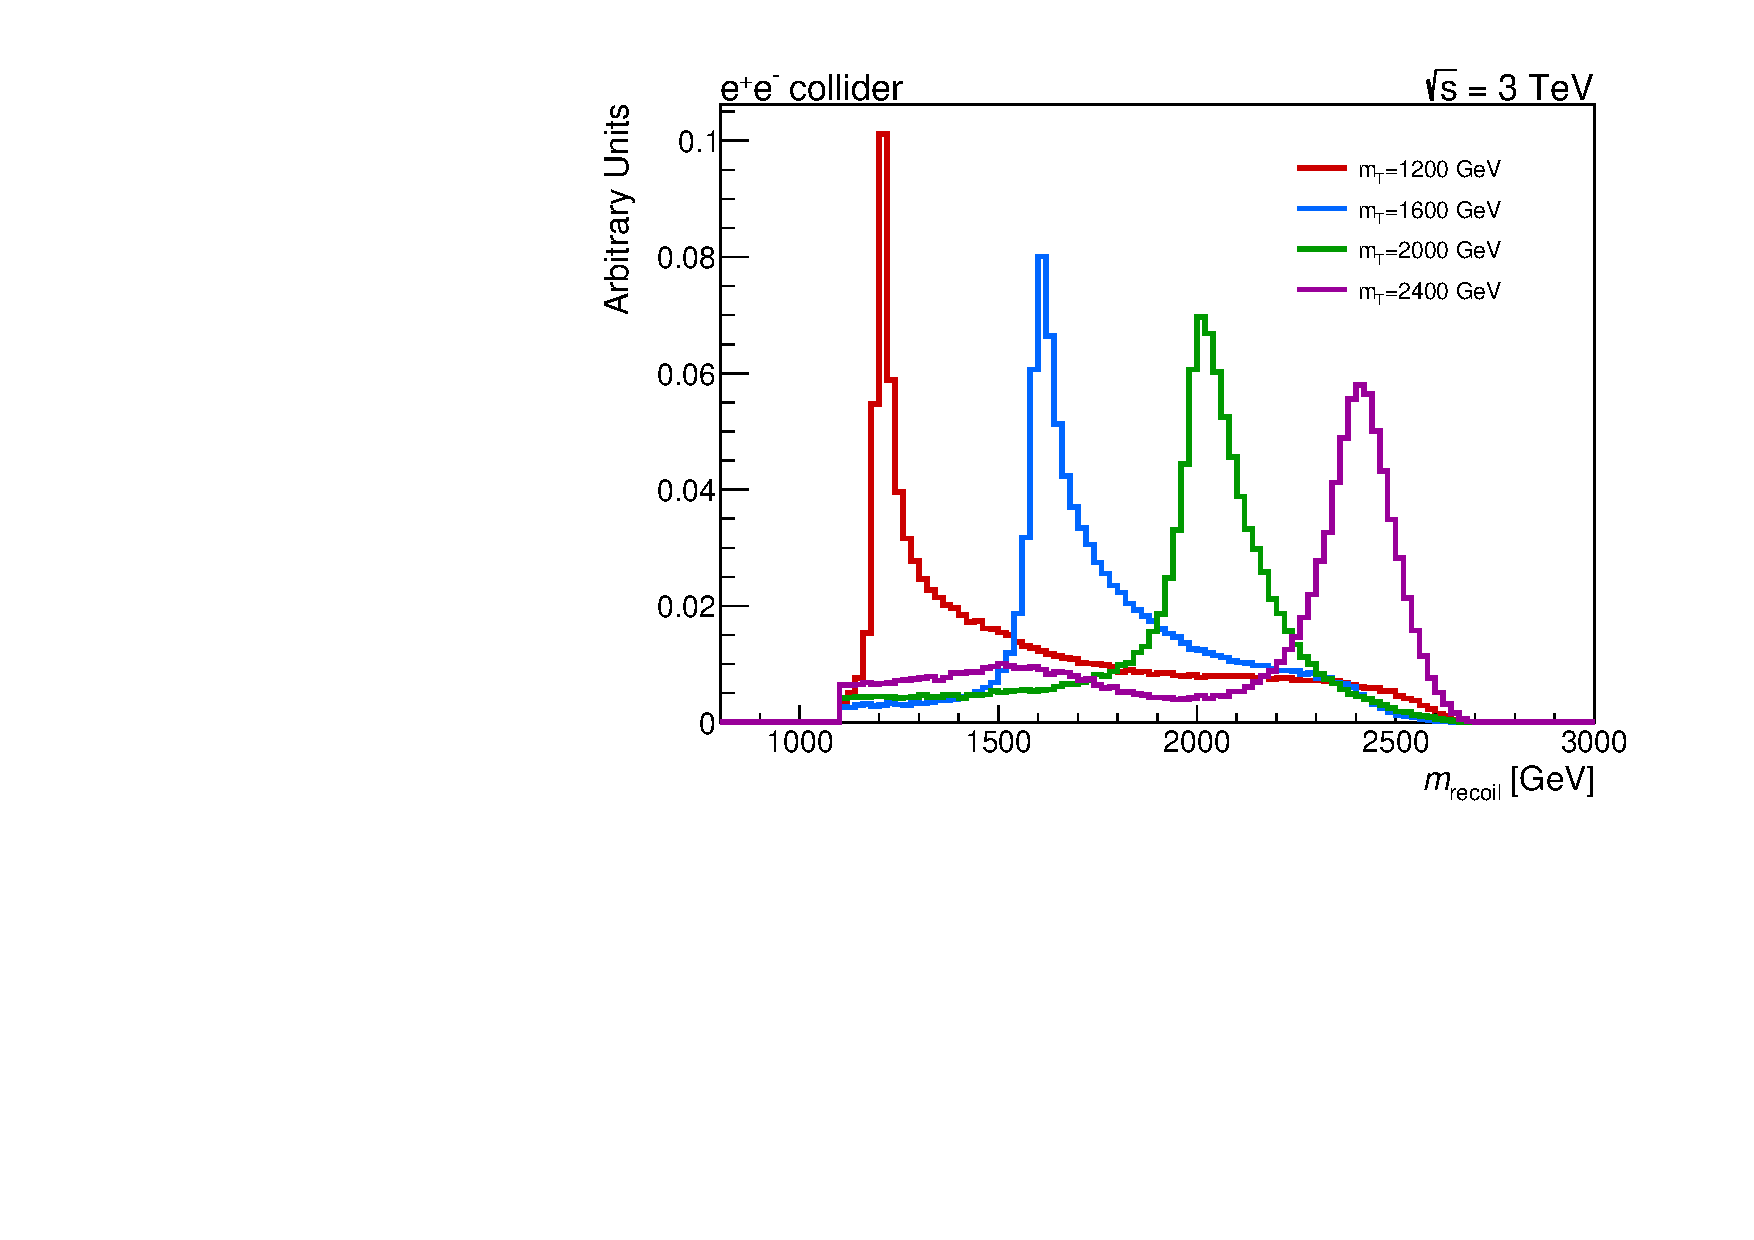
\includegraphics[width=0.78\textwidth]{signals_after_cuts.pdf}
\caption{Legacy recoil-mass shapes for the signal benchmarks after the reviewed
baseline selection.  The low-mass tail is used as a diagnostic of top-candidate
misassignment.}
\label{fig:signals}
\end{figure}

\begin{figure}[t]
\centering
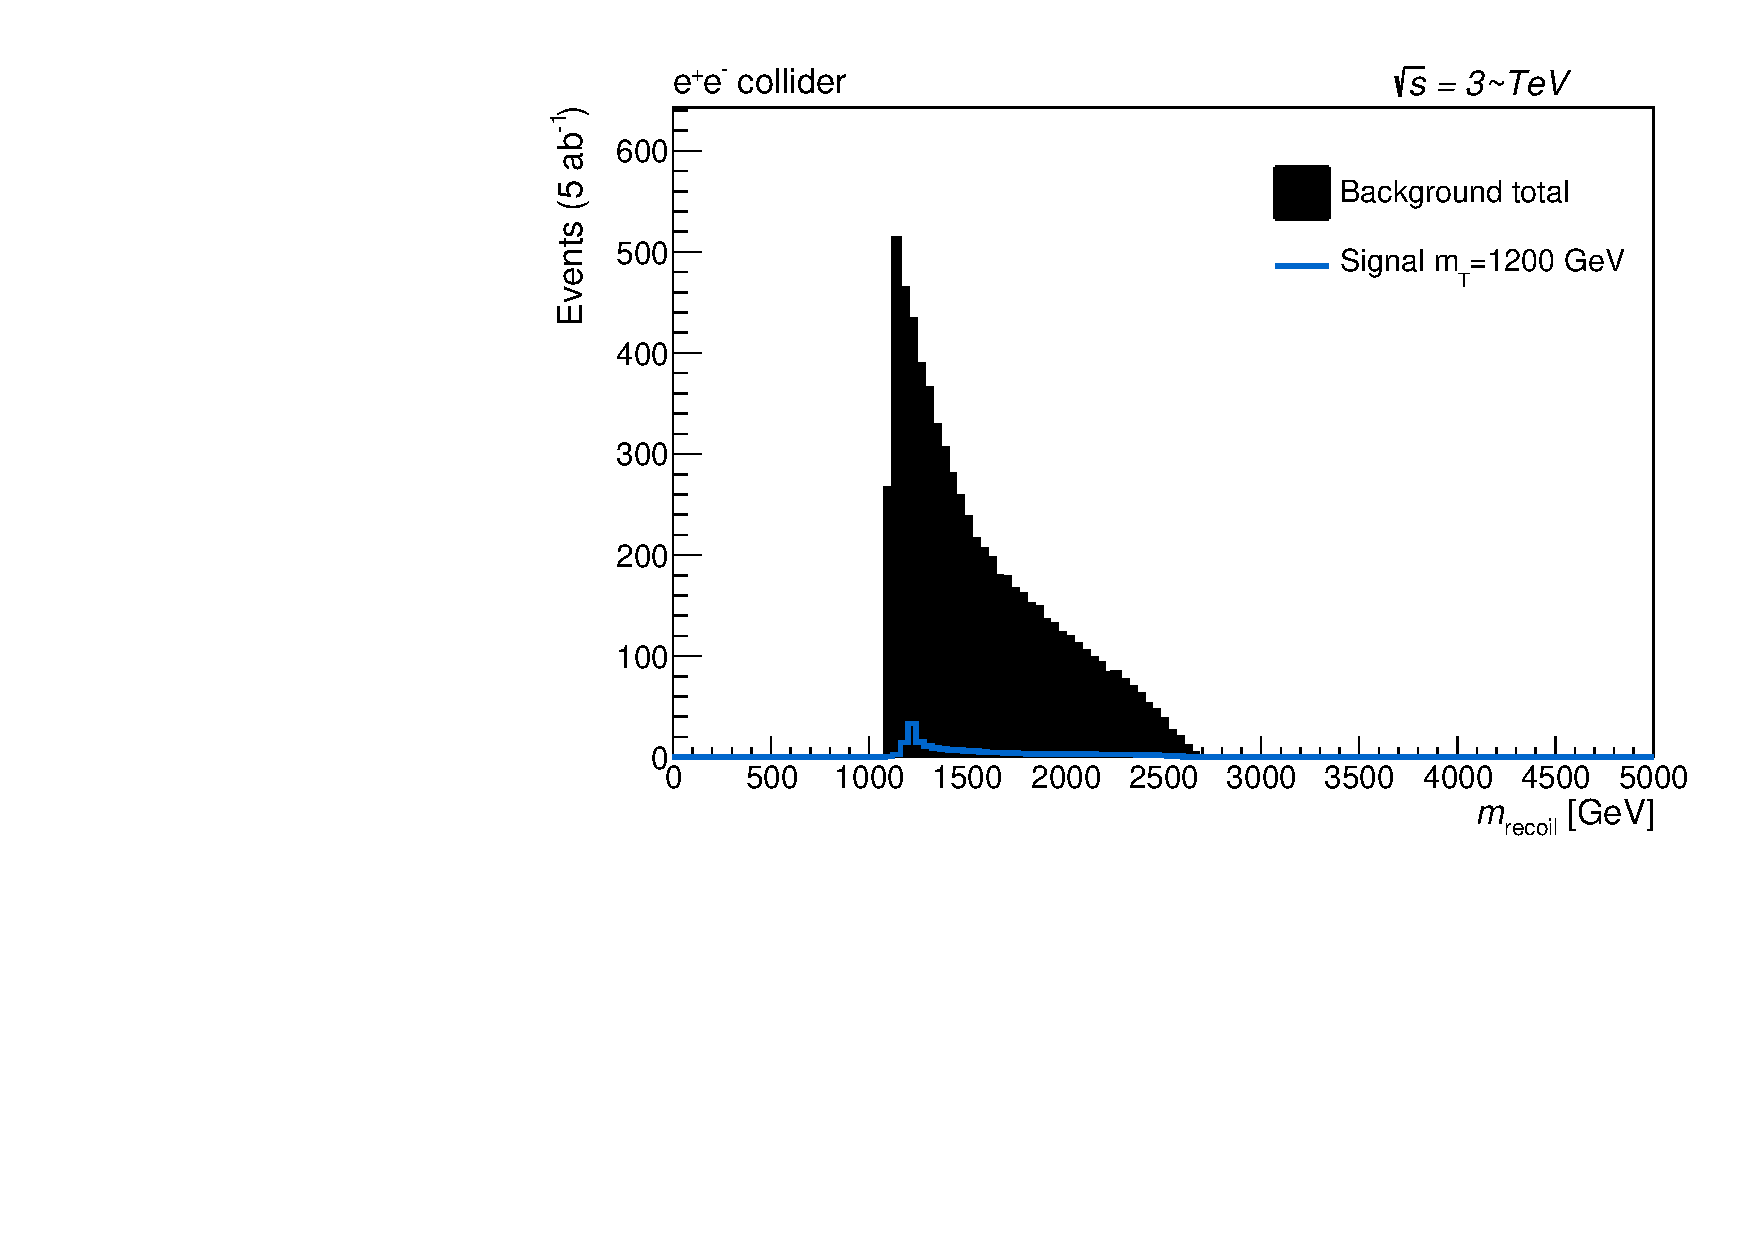
\includegraphics[width=0.78\textwidth]{recoil_baseline.pdf}
\caption{Legacy baseline recoil-mass spectrum for $m_T=\SI{1.2}{TeV}$ and
$\kappa_T=0.20$, normalized to $\SI{5}{ab^{-1}}$.}
\label{fig:baseline-recoil}
\end{figure}

\subsection{ISR and polarization}

The ISR and beam-polarization samples are used as stress tests.  The
right-handed electron-polarization sample reduces the dominant $t\bar t$
background relative to the left-handed sample, but ISR broadens the recoil
distribution and reduces the simple counting reach.  The revised paper does
not assume a luminosity split among polarization states; the three samples are
shown separately until a CLIC running scenario is imposed.

\begin{figure}[t]
\centering
\begin{minipage}{0.48\textwidth}
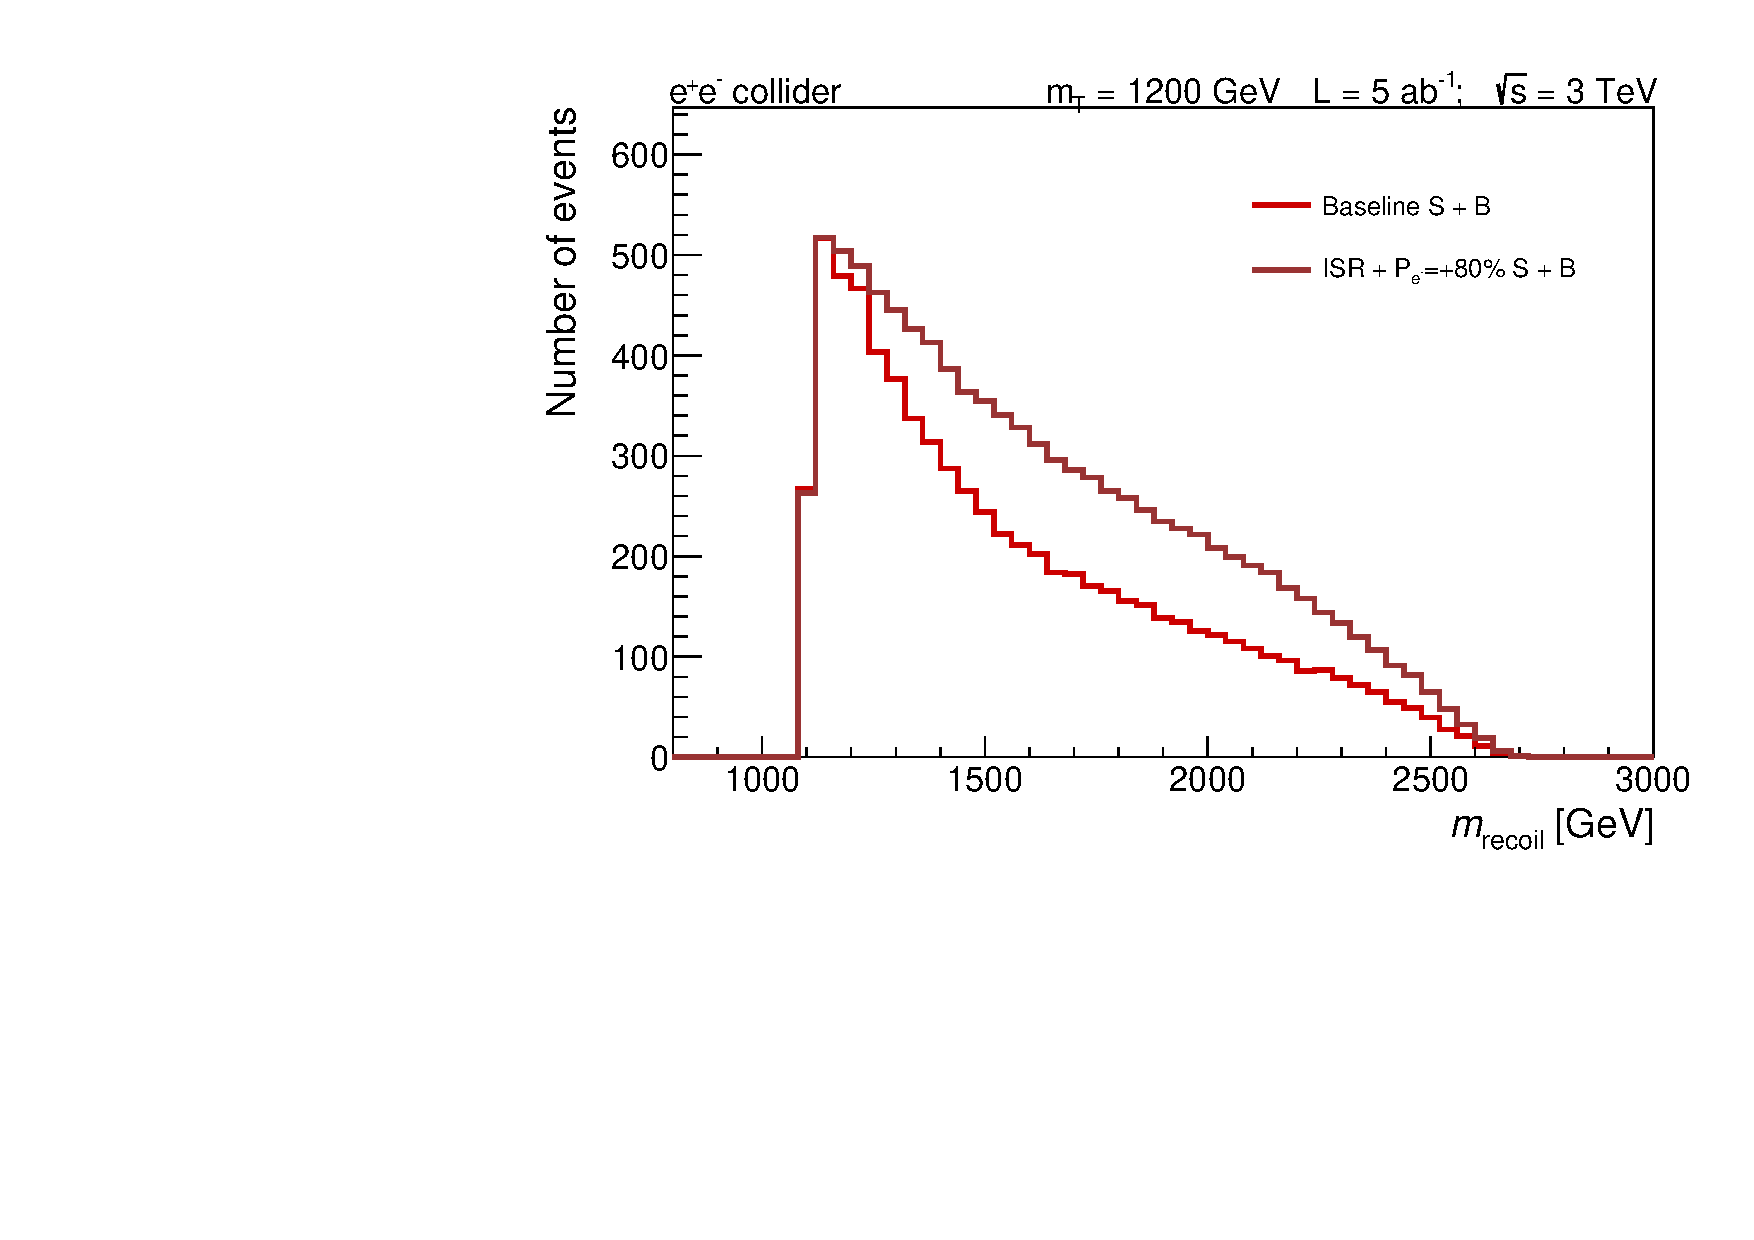
\includegraphics[width=\textwidth]{recoil_comparison_1200.pdf}
\end{minipage}
\begin{minipage}{0.48\textwidth}
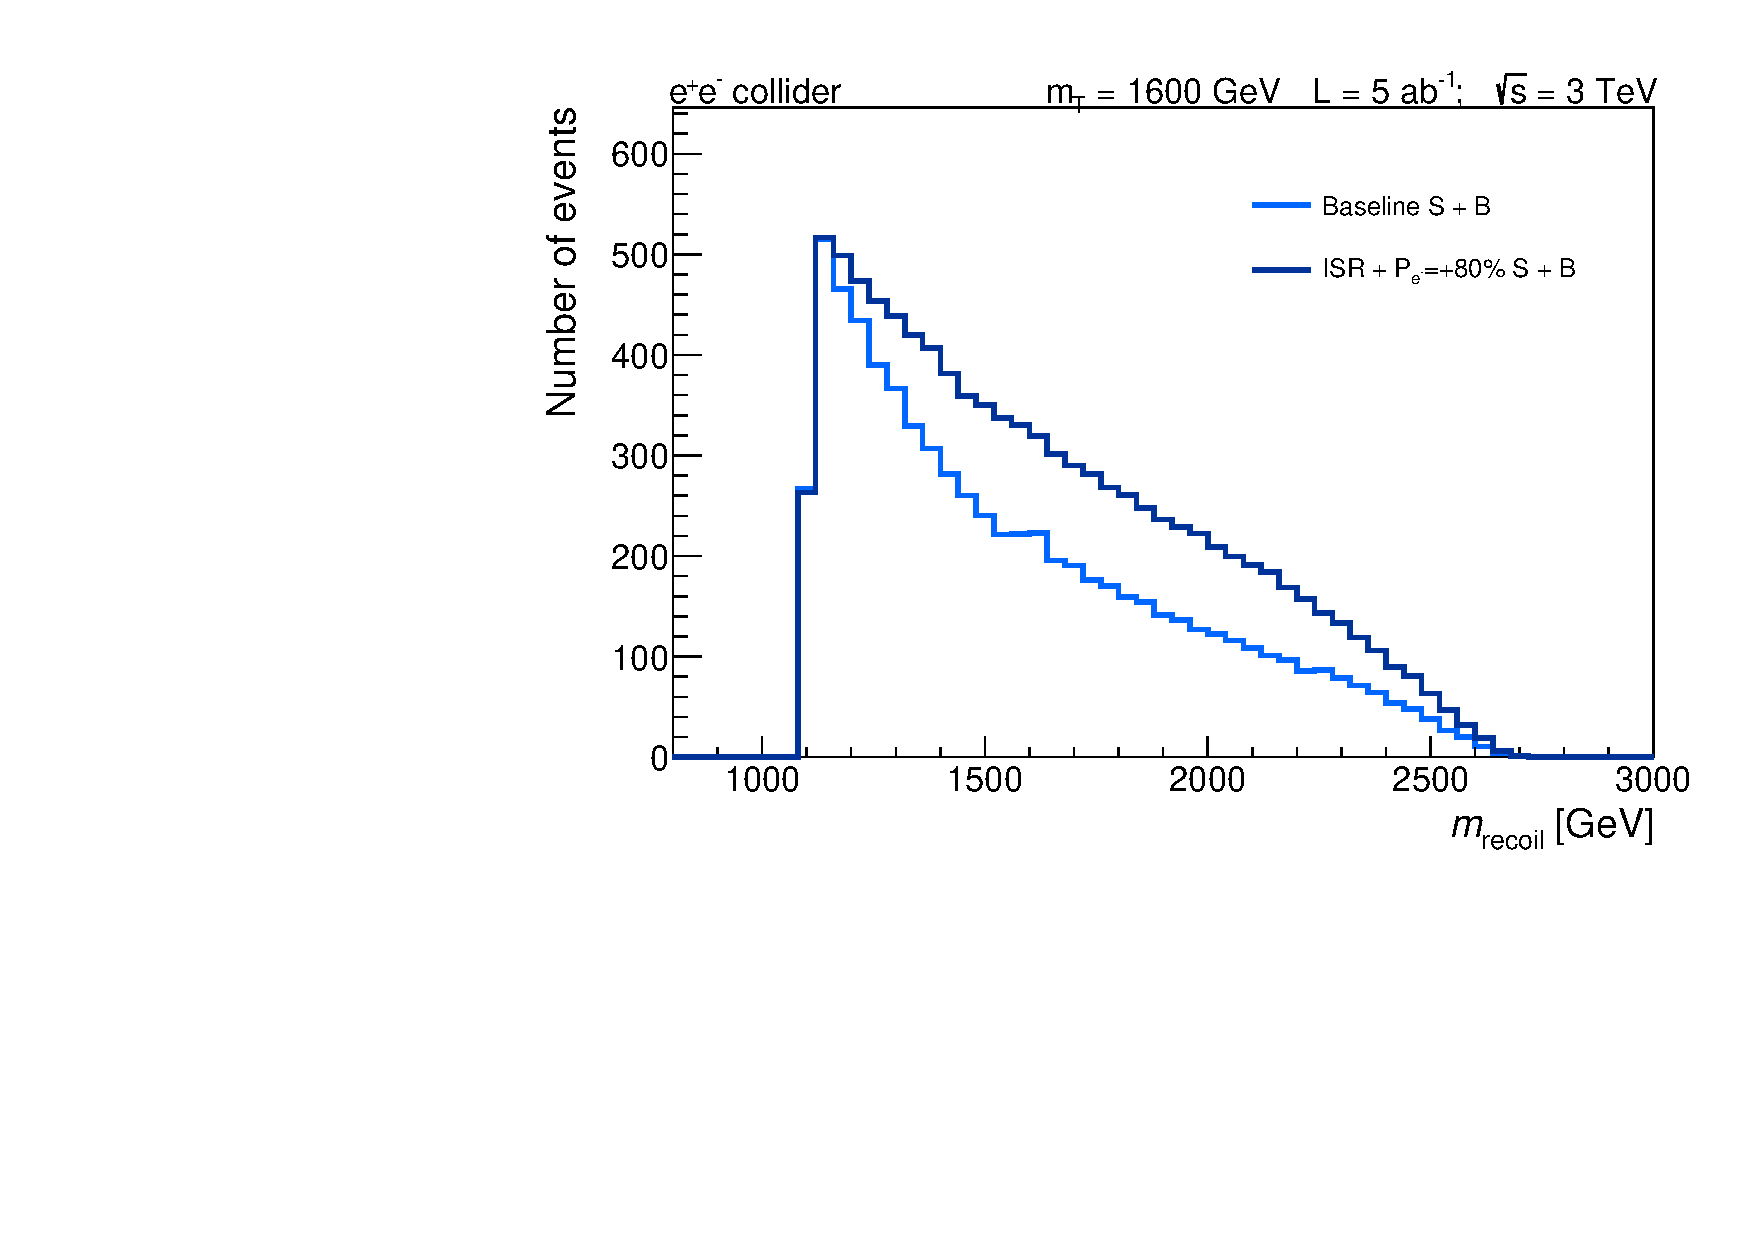
\includegraphics[width=\textwidth]{recoil_comparison_1600.pdf}
\end{minipage}
\begin{minipage}{0.48\textwidth}
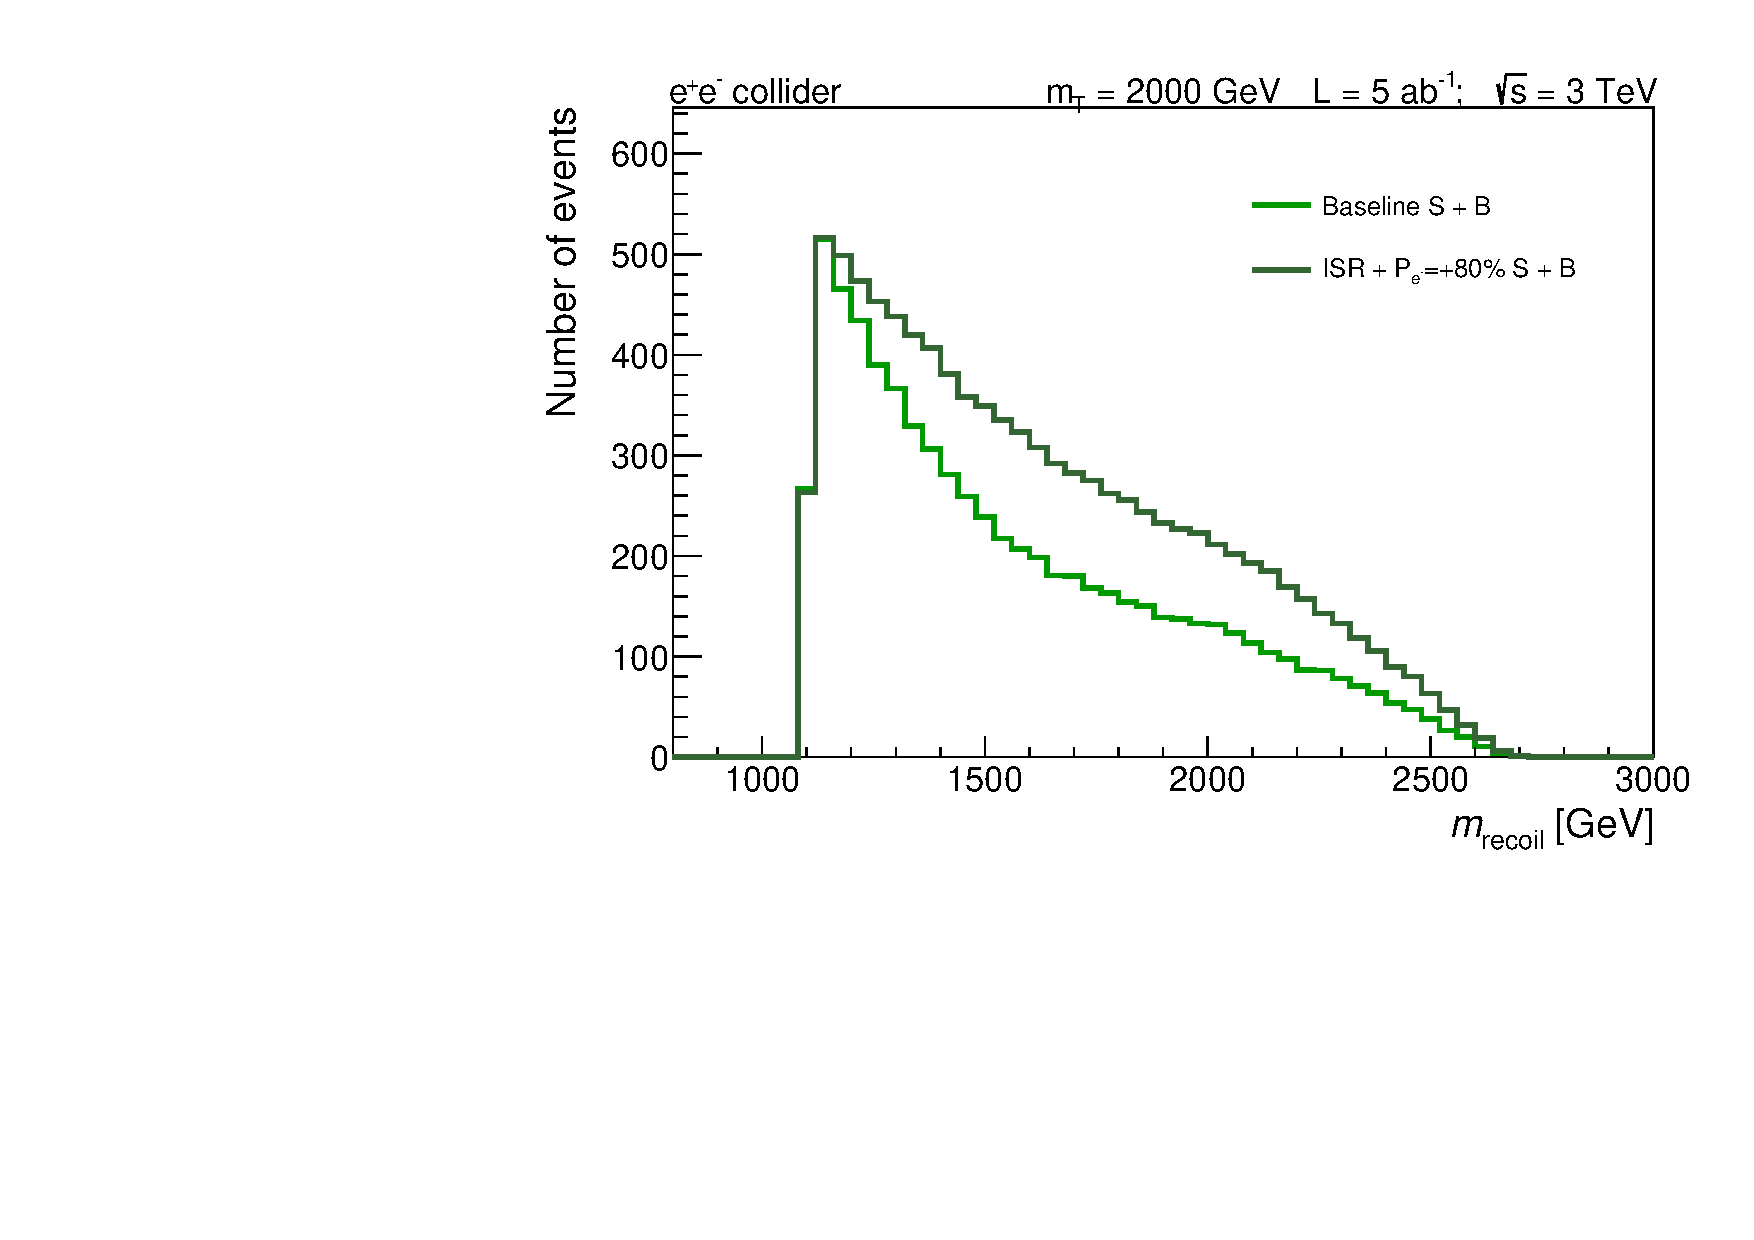
\includegraphics[width=\textwidth]{recoil_comparison_2000.pdf}
\end{minipage}
\begin{minipage}{0.48\textwidth}
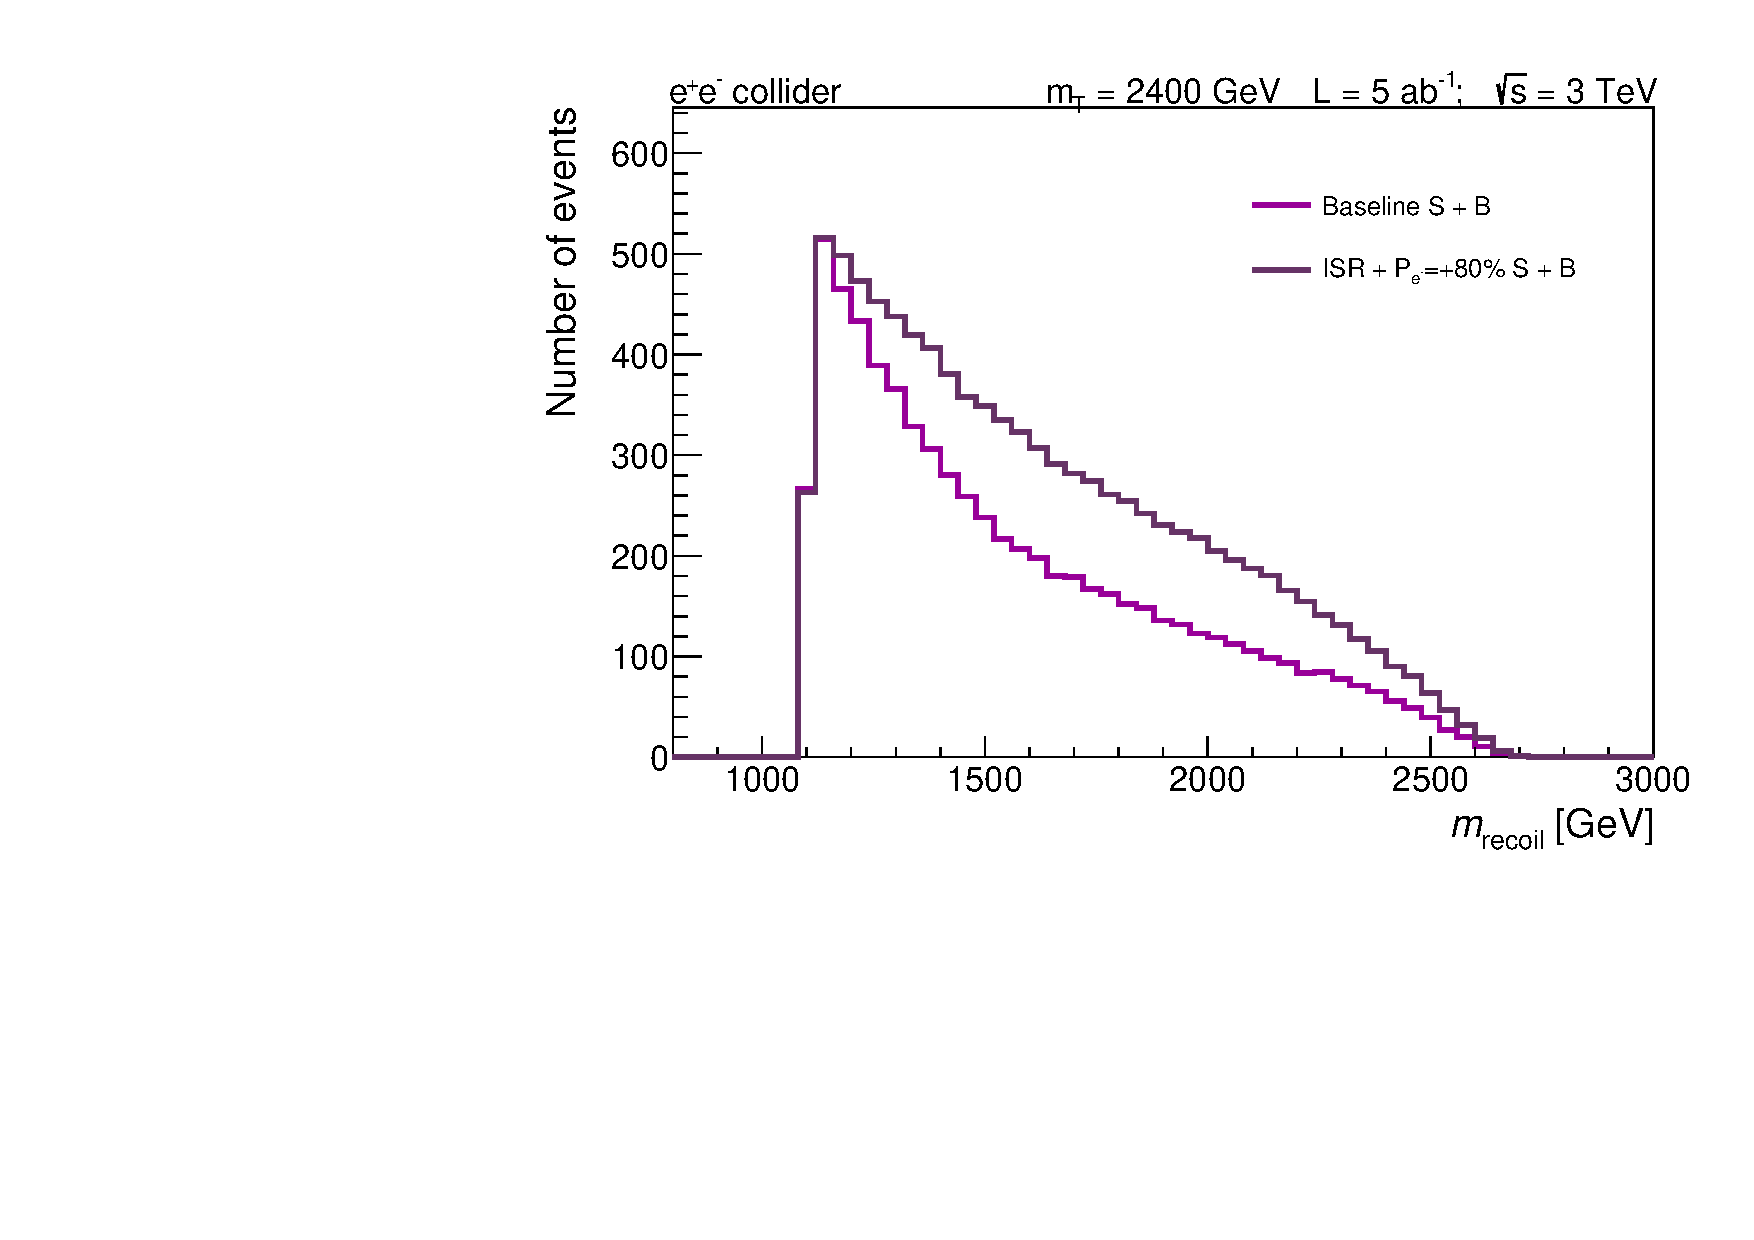
\includegraphics[width=\textwidth]{recoil_comparison_2400.pdf}
\end{minipage}
\caption{Legacy comparison of baseline and ISR+$P_{e^-}=+80\%$ signal-plus-background
recoil spectra for the four benchmark masses.}
\label{fig:recoil-comparison}
\end{figure}

\begin{table}[t]
\centering
\caption{Benchmark yields and significance cross-checks at $\kappa_T=0.20$.
The headline discovery test in the revised text uses the binned profile-likelihood workflow; the
last three columns provide transparent counting cross-checks with no nuisance parameters, a
$5\%$ background-normalization nuisance, and a conservative $10\%$ background plus $5\%$
signal-efficiency scenario.}
\label{tab:benchmark-yields}
\begin{tabular}{llrrrrrr}
\toprule
$m_T$ [TeV] & Scenario & $S$ & $B$ & $S/\sqrt{S+B}$ & $Z_A$ & $Z_A(5\%B)$ & $Z_A(10\%B,5\%S)$ \\
\midrule
    1.2 & baseline & 198.9 & 6939 & 2.35 & 2.38 & 0.55 & 0.27 \\
    1.2 & ISR+80 & 170.2 & 9707 & 1.71 & 1.72 & 0.34 & 0.16 \\
    1.2 & ISR-80 & 211.7 & 18575 & 1.54 & 1.55 & 0.22 & 0.11 \\
    1.6 & baseline & 165.6 & 6939 & 1.96 & 1.98 & 0.46 & 0.22 \\
    1.6 & ISR+80 & 130.8 & 9707 & 1.32 & 1.32 & 0.26 & 0.13 \\
    1.6 & ISR-80 & 160.5 & 18575 & 1.17 & 1.18 & 0.17 & 0.08 \\
    2.0 & baseline & 97.0 & 6939 & 1.16 & 1.16 & 0.27 & 0.13 \\
    2.0 & ISR+80 & 64.8 & 9707 & 0.66 & 0.66 & 0.13 & 0.06 \\
    2.0 & ISR-80 & 81.6 & 18575 & 0.60 & 0.60 & 0.09 & 0.04 \\
    2.4 & baseline & 25.6 & 6939 & 0.31 & 0.31 & 0.07 & 0.03 \\
    2.4 & ISR+80 & 14.5 & 9707 & 0.15 & 0.15 & 0.03 & 0.01 \\
    2.4 & ISR-80 & 18.0 & 18575 & 0.13 & 0.13 & 0.02 & 0.01 \\
\bottomrule
\end{tabular}
\end{table}


\subsection{Response to realism limitations}

The present numbers should be read as a controlled study of the recoil
observable, not as a full GEANT4/CLICdet projection.  The fresh production now
adds the CLIC luminosity-spectrum treatment and a parametric one-bunch
$\gamma\gamma\to$hadrons overlay stress test to the earlier ISR-only samples.
Detector granularity, resolutions, calibrated top-tag and b-tag efficiencies,
and the remaining high-priority backgrounds are still fast/parametric inputs
rather than full detector simulation.  The CLIC staged design and new-physics
studies~\cite{CLIC:2018fvx,CLICdp:2018esa} make clear that these machine effects
are part of the experimental environment at multi-TeV energy; Tables
\ref{tab:fresh-clic-sqrts}--\ref{tab:fresh-clic-vs-isr} therefore quote the new
machine-effect diagnostics explicitly.

\begin{table}[t]
\centering
\caption{Fresh CLIC luminosity-spectrum diagnostic for unpolarized signal
samples.  The table reports the generated effective collision energy
$\sqrt{s'}$, the longitudinal boost, and the 95th percentile of the recoil-mass
shift induced by using the nominal $\sqrt{s}=\SI{3}{TeV}$ in the recoil formula.}
\label{tab:fresh-clic-sqrts}
\small
\begin{tabular}{lrrrrrr}
\toprule
$m_T$ [TeV] & $\langle\sqrt{s'}\rangle$ [GeV] & $q_{5}$ [GeV] & $q_{50}$ [GeV]
& $f(\sqrt{s'}<0.95\sqrt{s})$ & $\langle|\beta_z|\rangle$ & $q_{95}(|\Delta m_{\rm rec}|)$ [GeV] \\
\midrule
    1.2 & 2782 & 1950 & 2968 & 0.342 & 0.072 & 1091 \\
    1.6 & 2862 & 2305 & 2982 & 0.269 & 0.044 & 718 \\
    2.0 & 2918 & 2588 & 2991 & 0.192 & 0.026 & 419 \\
    2.4 & 2962 & 2797 & 2997 & 0.084 & 0.012 & 204 \\
\bottomrule
\end{tabular}
\end{table}


\begin{table}[t]
\centering
\caption{Fresh CLIC luminosity-spectrum counting cross-checks at $\kappa_T=0.20$,
using the mass-matched BDT selection for each signal point and the four generated
background classes.  These numbers include ISR plus the CLIC luminosity-spectrum
sampling used in the fresh production, but not the overlay stress-test variant.}
\label{tab:fresh-clic-reach}
\small
\begin{tabular}{llrrrrrr}
\toprule
$m_T$ [TeV] & Beam & $S$ & $B$ & $S/\sqrt{S+B}$ & $Z_A$ & $Z_A(5\%B)$ & $Z_A(10\%B,5\%S)$ \\
\midrule
    1.2 & $P_{e^-}=-80\%$ & 195.5 & 13243.7 & 1.69 & 1.69 & 0.29 & 0.14 \\
    1.2 & unpol. & 178.2 & 10278.4 & 1.74 & 1.75 & 0.34 & 0.16 \\
    1.2 & $P_{e^-}=+80\%$ & 157.0 & 7133.3 & 1.84 & 1.85 & 0.43 & 0.21 \\
    1.6 & $P_{e^-}=-80\%$ & 135.6 & 8421.4 & 1.47 & 1.47 & 0.31 & 0.15 \\
    1.6 & unpol. & 129.5 & 6404.3 & 1.60 & 1.61 & 0.39 & 0.19 \\
    1.6 & $P_{e^-}=+80\%$ & 116.1 & 4300.8 & 1.75 & 1.76 & 0.51 & 0.25 \\
    2.0 & $P_{e^-}=-80\%$ & 71.8 & 6737.6 & 0.87 & 0.87 & 0.21 & 0.10 \\
    2.0 & unpol. & 64.6 & 5052.5 & 0.90 & 0.91 & 0.25 & 0.12 \\
    2.0 & $P_{e^-}=+80\%$ & 57.4 & 3470.6 & 0.97 & 0.97 & 0.31 & 0.15 \\
    2.4 & $P_{e^-}=-80\%$ & 14.6 & 5758.1 & 0.19 & 0.19 & 0.05 & 0.02 \\
    2.4 & unpol. & 13.5 & 4325.7 & 0.21 & 0.21 & 0.06 & 0.03 \\
    2.4 & $P_{e^-}=+80\%$ & 12.0 & 2820.3 & 0.23 & 0.23 & 0.08 & 0.04 \\
\bottomrule
\end{tabular}
\end{table}


\begin{table}[t]
\centering
\caption{Parametric $\gamma\gamma\to$hadrons overlay stress test for the
unpolarized fresh CLIC samples.  Ratios are overlay divided by the corresponding
clean luminosity-spectrum reconstruction after the mass-matched BDT selection.}
\label{tab:fresh-clic-overlay}
\small
\begin{tabular}{lrrrrrrr}
\toprule
$m_T$ [TeV] & $S_{\rm clean}$ & $S_{\rm ov}$ & $S_{\rm ov}/S_{\rm clean}$
& $B_{\rm clean}$ & $B_{\rm ov}$ & $B_{\rm ov}/B_{\rm clean}$ & $Z_{\rm ov}/Z_{\rm clean}$ \\
\midrule
    1.2 & 178.2 & 178.1 & 0.999 & 10278.4 & 10229.7 & 0.995 & 1.002 \\
    1.6 & 129.5 & 128.9 & 0.995 & 6404.3 & 6356.6 & 0.993 & 0.999 \\
    2.0 & 64.6 & 64.0 & 0.991 & 5052.5 & 4973.2 & 0.984 & 0.999 \\
    2.4 & 13.5 & 13.3 & 0.986 & 4325.7 & 4249.0 & 0.982 & 0.995 \\
\bottomrule
\end{tabular}
\end{table}


\begin{table}[t]
\centering
\caption{Impact of replacing the ISR-only lepton beams by the fresh CLIC
luminosity-spectrum setup for unpolarized samples.  Ratios compare the
mass-matched BDT yields from the fresh CLIC run to the older ISR-only run.}
\label{tab:fresh-clic-vs-isr}
\small
\begin{tabular}{lrrrrr}
\toprule
$m_T$ [TeV] & $S_{\rm CLIC}/S_{\rm ISR}$ & $B_{\rm CLIC}/B_{\rm ISR}$
& $Z_{\rm ISR}$ & $Z_{\rm CLIC}$ & $Z_{\rm CLIC}/Z_{\rm ISR}$ \\
\midrule
    1.2 & 0.962 & 1.059 & 1.87 & 1.75 & 0.935 \\
    1.6 & 0.969 & 1.082 & 1.73 & 1.61 & 0.932 \\
    2.0 & 0.966 & 1.094 & 0.98 & 0.91 & 0.924 \\
    2.4 & 0.970 & 1.037 & 0.22 & 0.21 & 0.953 \\
\bottomrule
\end{tabular}
\end{table}


\section{Scanning \texorpdfstring{$\kappa_T$}{kappaT}}
\label{sec:kappa}

The $\kappa_T$ scan is reinterpreted with a finite-width validity criterion.
Only points with $\Gamma_T/m_T\le10\%$ are used for the main narrow-resonance
reach discussion.  Larger-width samples are not called unphysical.  They are
outside the domain where narrow-width production plus \textsc{MadSpin} decays
can be used as a standalone estimate without an interference-aware
matrix-element study.

\begin{table}[t]
\centering
\caption{Nominal validity domain used for the main $(m_T,\kappa_T)$ interpretation.
Points above $\Gamma_T/m_T=10\%$ are not interpreted as narrow-resonance reach points.}
\label{tab:width-validity-summary}
\begin{tabular}{cccl}
\toprule
$m_T$ [TeV] & Largest kept $\kappa_T$ & First omitted $\kappa_T$ & Criterion \\
\midrule
    1.2 & 0.45 & 0.50 & $\Gamma_T/m_T \le 10\%$ \\
    1.6 & 0.30 & 0.35 & $\Gamma_T/m_T \le 10\%$ \\
    2.0 & 0.25 & 0.30 & $\Gamma_T/m_T \le 10\%$ \\
    2.4 & 0.20 & 0.25 & $\Gamma_T/m_T \le 10\%$ \\
\bottomrule
\end{tabular}
\end{table}


\begin{figure}[t]
\centering
\begin{minipage}{0.32\textwidth}
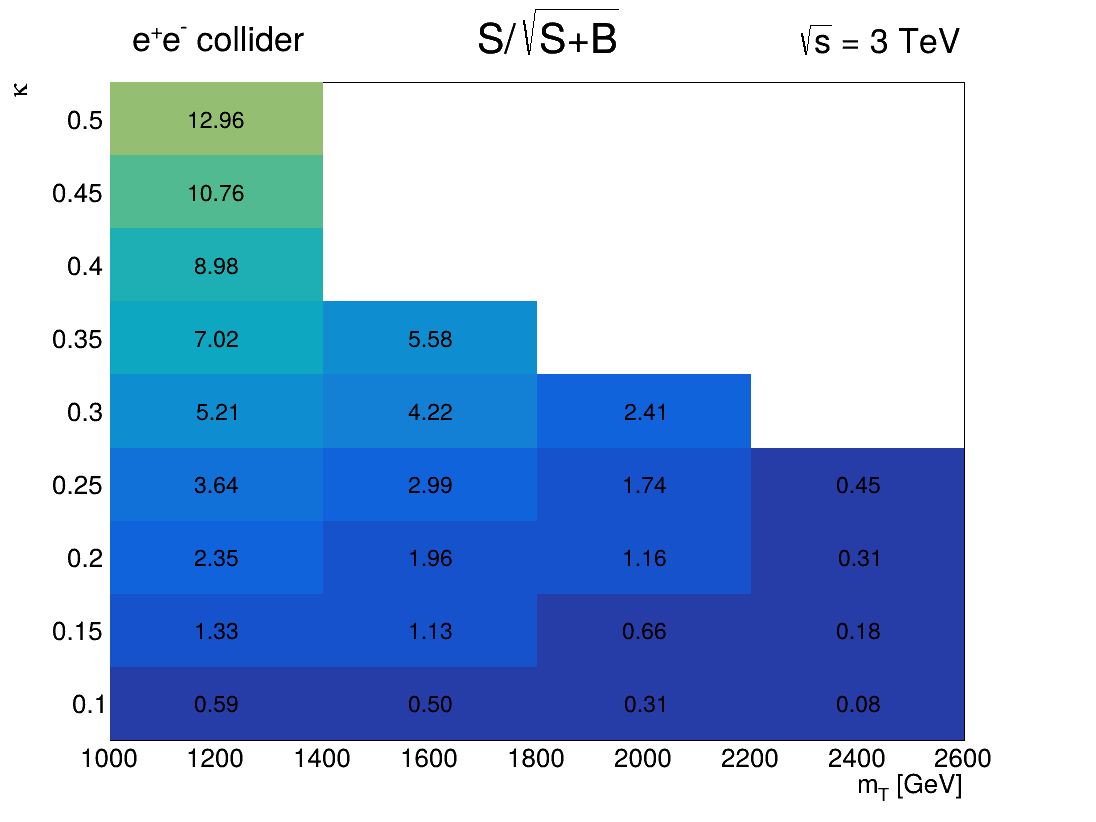
\includegraphics[width=\textwidth]{kappa_scan_baseline.png}
\end{minipage}
\begin{minipage}{0.32\textwidth}
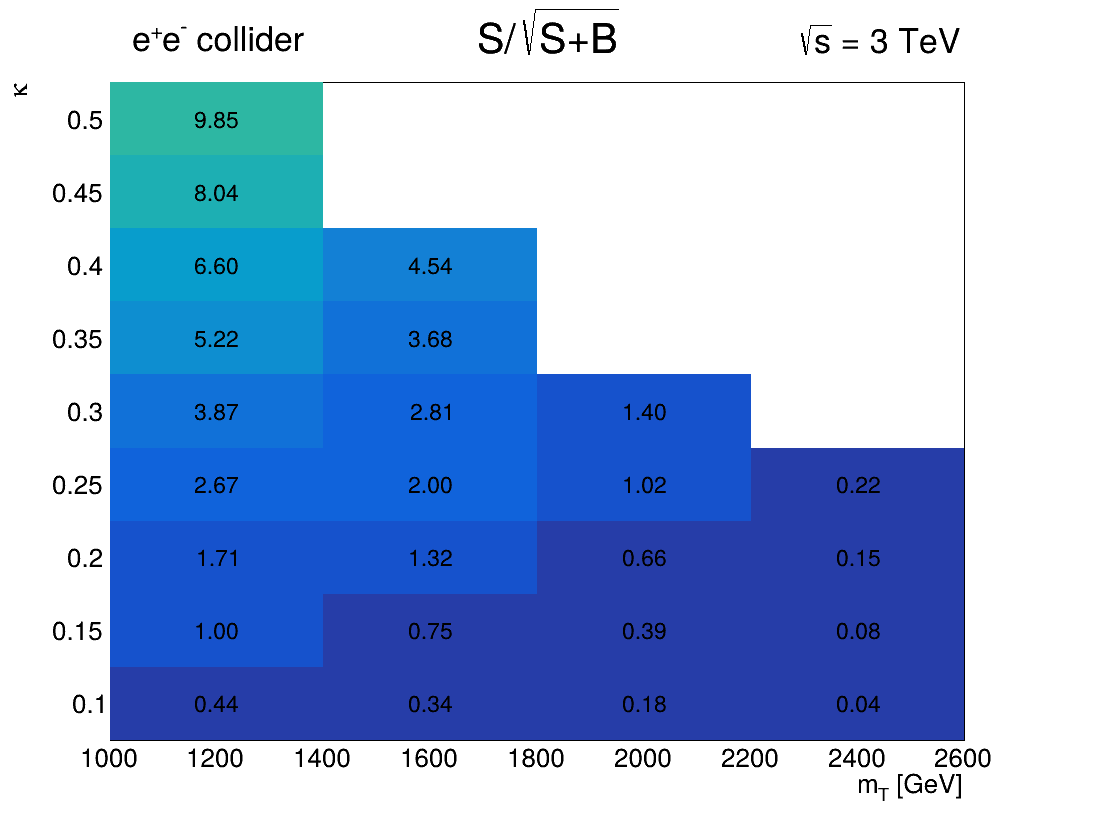
\includegraphics[width=\textwidth]{kappa_scan_plus80ISR.png}
\end{minipage}
\begin{minipage}{0.32\textwidth}
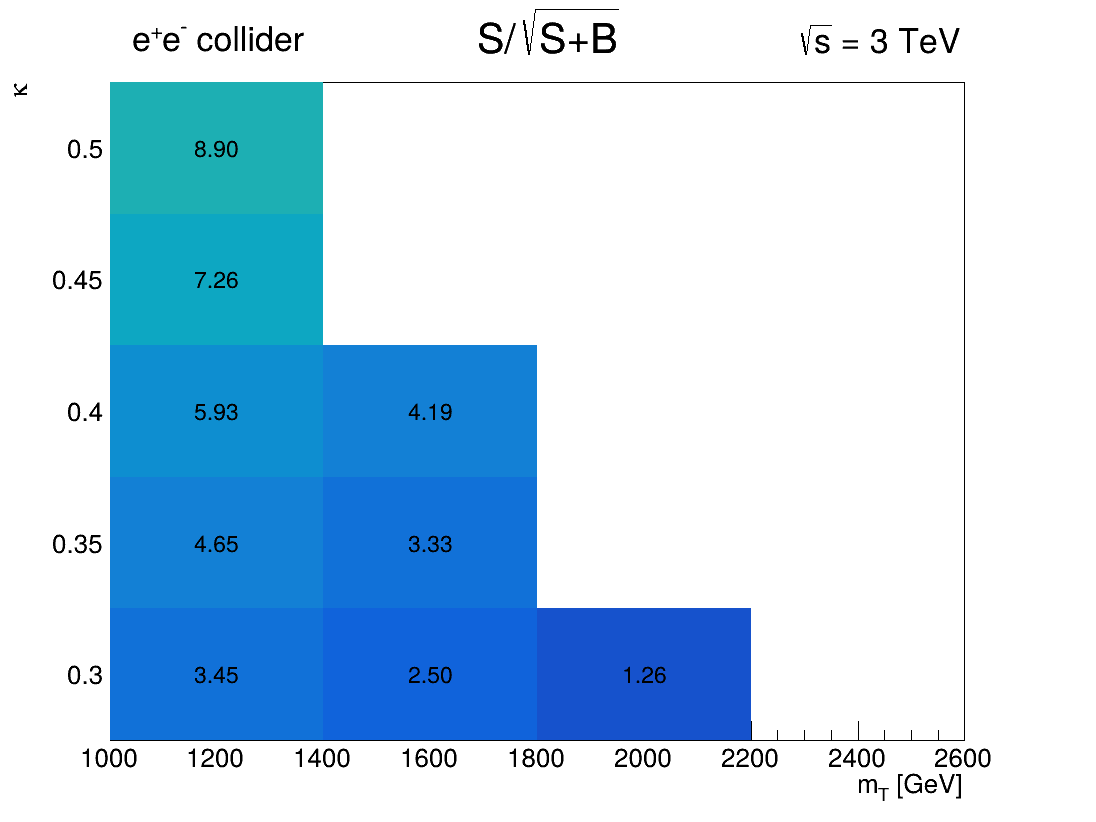
\includegraphics[width=\textwidth]{kappa_scan_minus80ISR.png}
\end{minipage}
\caption{Existing $(m_T,\kappa_T)$ counting-significance maps for the legacy
baseline, ISR+$P_{e^-}=+80\%$, and ISR+$P_{e^-}=-80\%$ samples.  The
interpretation is restricted by Table~\ref{tab:width-validity-summary}; points
above the width threshold require an interference-aware treatment.}
\label{fig:kappa-scans}
\end{figure}

The representative wide-point validation to add is a full final-state
matrix-element sample near the boundary, for example $m_T=\SI{2.0}{TeV}$ and
$\kappa_T=0.25$ or $m_T=\SI{1.6}{TeV}$ and $\kappa_T=0.30$.  This stress test
should compare the recoil line shape and normalization to the current
production-times-decay/MadSpin sample.  If the difference is larger than the
statistical uncertainty assigned to the reach map, the high-width region must
be shown only as a qualitative sensitivity guide.

\section{Comparison with related work}
\label{sec:comparison}

Current LHC searches directly constrain single production of vector-like quarks
in dedicated channels such as $T\to Ht/Zt$ and $Q\to Wb$
\cite{ATLAS:2023nqh,ATLAS:2025wbl,CMS:B2G22004}.  Those analyses use the
large LHC production rate and mature detector performance, but their strongest
regions are necessarily tied to final-state assumptions.  The present study
does not claim stronger absolute reach in the $\kappa_T$--$m_T$ plane.  Its
role is complementary: it tests whether a lepton collider can provide a
decay-agnostic recoil observable that can later be combined with channel
specific selections.

The result is also complementary to CLIC phenomenology studies targeting
specific $T$ or $B$ decay modes~\cite{Han:2022exx,Han:2022mzp}.  Those studies
can optimize for a known final state; the recoil strategy deliberately trades
some raw sensitivity for reduced branching-fraction dependence.  A final
paper-quality comparison should therefore quote both axes: absolute reach after
realistic detector effects, and stability of the efficiency under forced
$Wb$, $Zt$, and $Ht$ decay modes.

\section{Discussion and outlook}
\label{sec:outlook}

The recoil-mass technique remains the central physics argument.  In an
$e^+e^-$ environment, reconstructing the associated hadronic top gives direct
access to the mass scale of the system recoiling against it, even when the
heavy partner decay is not fully reconstructed.  This is precisely the handle
that complements channel-dependent LHC searches.

The current study also shows where the method is fragile.  ISR and beam-energy
loss smear the recoil mass because Eq.~\eqref{eq:recoilmass} uses the nominal
collision energy.  Beamstrahlung and $\gamma\gamma\to$hadrons overlay are
therefore not secondary details; they are part of the observable definition.
Promising mitigation variables are global and decay-agnostic: recoil-system
transverse-momentum imbalance, top--recoil acolinearity, event thrust, and
forward missing momentum.  These variables should enter the next binned
likelihood or multivariate analysis before claiming CLIC-realistic discovery
reach.

The next production campaign has a clear checklist: rerun the nominal
$|\eta|<2.5$ selection; include the expanded background set; add a CLIC beam
spectrum and overlay stress test; replace truth $b$-matching with calibrated
efficiencies and mistags; run forced $T\to Wb$, $Zt$, and $Ht$ samples; and
validate at least one finite-width boundary point with a full matrix-element
sample.  With those ingredients, the recoil approach can become a reusable
baseline for model-reinterpretation studies of vector-like top partners at
future lepton colliders.

\appendix

\section{Width ratios}
\label{app:widths}
\begin{table}[p]
\centering
\caption{Width ratios used to define the scan validity domain.}
\label{tab:width-ratios}
\begin{tabular}{ccrcl}
\toprule
$m_T$ [TeV] & $\kappa_T$ & $\Gamma_T$ [GeV] & $\Gamma_T/m_T$ [\%] & Main-scan status \\
\midrule
    1.2 & 0.10 & 5.580 & 0.5 & kept \\
    1.2 & 0.15 & 12.554 & 1.0 & kept \\
    1.2 & 0.20 & 22.318 & 1.9 & kept \\
    1.2 & 0.25 & 34.872 & 2.9 & kept \\
    1.2 & 0.30 & 50.215 & 4.2 & kept \\
    1.2 & 0.35 & 68.349 & 5.7 & kept \\
    1.2 & 0.40 & 89.272 & 7.4 & kept \\
    1.2 & 0.45 & 112.984 & 9.4 & kept \\
    1.2 & 0.50 & 139.487 & 11.6 & outside \\
    1.2 & 0.55 & 168.779 & 14.1 & outside \\
    1.2 & 0.60 & 200.858 & 16.7 & outside \\
    1.2 & 0.65 & 235.735 & 19.6 & outside \\
    1.2 & 0.70 & 273.396 & 22.8 & outside \\
    1.2 & 0.75 & 313.848 & 26.2 & outside \\
    1.6 & 0.10 & 13.318 & 0.8 & kept \\
    1.6 & 0.15 & 29.965 & 1.9 & kept \\
    1.6 & 0.20 & 53.271 & 3.3 & kept \\
    1.6 & 0.25 & 83.236 & 5.2 & kept \\
    1.6 & 0.30 & 119.859 & 7.5 & kept \\
    1.6 & 0.35 & 163.142 & 10.2 & outside \\
    1.6 & 0.40 & 213.079 & 13.3 & outside \\
    1.6 & 0.45 & 269.687 & 16.9 & outside \\
    2.0 & 0.10 & 26.095 & 1.3 & kept \\
    2.0 & 0.15 & 58.714 & 2.9 & kept \\
    2.0 & 0.20 & 104.380 & 5.2 & kept \\
    2.0 & 0.25 & 163.093 & 8.2 & kept \\
    2.0 & 0.30 & 234.856 & 11.7 & outside \\
    2.0 & 0.35 & 319.658 & 16.0 & outside \\
    2.0 & 0.40 & 417.510 & 20.9 & outside \\
    2.4 & 0.10 & 45.171 & 1.9 & kept \\
    2.4 & 0.15 & 101.634 & 4.2 & kept \\
    2.4 & 0.20 & 180.682 & 7.5 & kept \\
    2.4 & 0.25 & 282.319 & 11.8 & outside \\
    2.4 & 0.30 & 406.530 & 16.9 & outside \\
\bottomrule
\end{tabular}
\end{table}


\section{Reviewer-response matrix and validation backlog}
\label{app:response}
\begin{table}[p]
\centering
\caption{Reviewer-response matrix implemented in the revised manuscript.}
\label{tab:response-matrix}
\small
\begin{tabular}{r p{0.23\linewidth} p{0.24\linewidth} p{0.38\linewidth}}
\toprule
\# & Review issue & Where addressed & Action \\
\midrule
    1 & Meaning of fully simulated & Secs. \ref{sec:samples}, \ref{sec:realism} & Term removed; detector treatment stated as fast/parametric unless GEANT4/CLICdet is added. \\
    2 & Top/b-tag efficiencies and mistags & Sec. \ref{sec:selection}, App. \ref{app:response} & Object definitions fixed; performance table is an explicit required validation item. \\
    3 & Isolation-veto definition & Sec. \ref{sec:selection} & Cone, thresholds, nearby-activity veto, and relative-$H_T$ logic documented. \\
    4 & Polarization choice & Sec. \ref{sec:realism} & Both $+80\%$ and $-80\%$ samples are shown; luminosity sharing is not assumed until a CLIC run plan is selected. \\
    5 & Background completeness & Table \ref{tab:background-status} & Included, locally available, and missing background classes separated. \\
    6 & Cutflow and normalization & Tables \ref{tab:reproducibility}, \ref{tab:benchmark-yields} & Yields trace back to ROOT histogram entries, cross sections, simulated events, and luminosity. \\
    7 & Finite widths/interference & Sec. \ref{sec:kappa}, Table \ref{tab:width-validity-summary} & Main scan restricted to $\Gamma_T/m_T\le10\%$; one full-matrix-element stress test listed as required. \\
    8 & Likelihood and systematics & Sec. \ref{sec:statistics}, Table \ref{tab:benchmark-yields} & Binned profile-likelihood workflow repaired; counting nuisance cross-checks included. \\
    9 & Modern taggers/ML & Sec. \ref{sec:outlook} & Presented as next analysis step; no unvalidated ML gain claimed. \\
    10 & Forced decay modes & App. \ref{app:response} & Validation matrix specified for $Wb$, $Zt$, and $Ht$ at 1.2 and 2.0 TeV. \\
\bottomrule
\end{tabular}
\end{table}


The forced-decay validation backlog is fixed to six samples:
$(m_T,\kappa_T)=(1.2~{\rm TeV},0.20)$ and $(2.0~{\rm TeV},0.20)$, each with
$T\to Wb$, $T\to Zt$, and $T\to Ht$.  For each sample the revision must report
the full cutflow, recoil peak position and width, final efficiency, and the
ratio of the efficiency to the inclusive sample.  The decay-agnostic wording is
kept only if these ratios are stable within the assigned systematic
uncertainty; otherwise the paper must use the weaker phrase
``decay-mode-tolerant''.

\bibliographystyle{JHEP}
\bibliography{references}

\end{document}
